\documentclass[aps,prd,twocolumn,superscriptaddress,nofootinbib,floatfix]{revtex4-2}
\usepackage{graphicx}
\usepackage{amsmath}
\usepackage{longtable}
\usepackage[colorlinks=true,linkcolor=blue,citecolor=blue,urlcolor=blue]{hyperref}

\newcommand{\Mah}{M_{\rm AH}}
\newcommand{\noterun}{\texttt{core-20261123-020543-eb1cd2a}}


\begin{document}

\title{A shared particle-in-cell implementation of Einstein--Vlasov matter in AthenaK:\\
releases and verification ladder}

\author{The shared implementation (core) of a cosmology program}
\date{Working note for gate G2, 21 November 2026}

\begin{abstract}
Six cosmology projects build on one implementation that couples collisionless matter,
sampled by particles, to the Z4c evolution of the spacetime in the AthenaK framework.
This note describes that implementation, what each of four releases added to it at the
request of the projects, and how far it is verified. On a fixed Kerr black hole both
particle pushers conserve the constants of geodesic motion to the level of the source
paper and converge at second order. A collapsing dust ball forms a black hole whose
horizon mass matches the initial mass at the paper's level when the horizon forms and
departs slightly from it later. A prolate spheroid forms its horizon at the paper's
time, with a mass deficit that shrinks with resolution. The five relativistic star
clusters of the paper reach the paper's fates. The bisection of their stability
threshold found no collapse on a coarse mesh; on a mesh twice as fine, with unkicked
controls, it brackets the threshold between two models just above the turning point of
the binding energy and well above it, and its next level is running. A
verifier with no part in the work recomputed a sample of the claims from raw outputs;
it confirmed the numbers and corrected one general statement about restarts. Two rows
of the ladder remain partial, and two limits of the gauge are scheduled for the next
release.
\end{abstract}

\maketitle

\section{Introduction}

Particle-in-cell methods for the Einstein--Vlasov system follow collisionless matter
with particles that move on geodesics of an evolving spacetime and deposit their
stress-energy on the mesh that evolves the metric~\cite{Wu:2026pic}. The method of
Ref.~\cite{Wu:2026pic} lives inside AthenaK~\cite{2026ApJS..283...27S}, whose
numerical-relativity module evolves the Z4c system with moving punctures and adaptive
refinement~\cite{Zhu:2024utz}. A program of six cosmology projects uses one shared copy
of this coupling, maintained in one source tree: primordial black holes and
gravitational waves in an early matter era, the collapse of a self-interacting core,
the growth of a black hole in a dark-matter dress, stochastic inflation, and the Hills
mechanism. Each project specifies what it needs and checks it; the shared
implementation builds it, tests it and releases it.

This note is the verification report of the shared implementation. Section~\ref{sec:impl}
describes the base coupling and the four releases that followed it.
Section~\ref{sec:ladder} goes through the verification ladder, the tests the program's
brief assigns to the shared implementation, row by row, with the evidence and what is
still partial. Section~\ref{sec:limits} lists the limits that are known and scheduled.
Every number behind a statement is in the ledger of Appendix~\ref{app:ledger}, with the
registered run or the source line it comes from, and with the claim of the independent
verifier where that verifier recomputed it.

\section{The shared implementation}\label{sec:impl}

\subsection{The base coupling}

A particle carries its position and its covariant spatial momentum per unit mass, $u_i$,
in the $3+1$ split with lapse $\alpha$, shift $\beta^i$ and spatial metric
$\gamma_{ij}$. Two pushers advance it: an implicit midpoint rule and a spacetime Boris
rule with two choices of tetrad. The metric and its first derivatives reach the particle
through Catmull--Rom or cubic-spline interpolation of the mesh fields. Each particle
deposits its energy density, momentum density and spatial stress with a cloud of
second, third or fourth order; an optional binomial filter with compensation smooths the
result, and the deposit across refinement levels conserves the integrated sources. The
deposited sources enter the matter terms of Z4c. Particles inside an apparent horizon,
or where the lapse falls below a bound, are removed with their mass and momentum on
record. A periodic domain with a conformal-time lapse, sources in density form and a
step limited by the expansion serve the cosmological set-ups. This base was tagged twice
before the program began its own releases.

\subsection{Four releases}

Figure~\ref{fig:arch} shows the implementation by release, with the gates of the shared
implementation above it. The first release of the program (core-v0.3) added
counter-based random numbers that repeat on processors, cards and the Python twin;
relativistic Monte Carlo collisions in the frame of the normal observer of each cell; a
scalar field evolved with Z4c with stochastic sources; spherical initial data with
extrinsic curvature; Bowen--York punctures with momentum and spin; and a Newtonian mode
in which the same particles feel a multigrid potential. The second (core-v0.4) added
linear gravitational waves of any wave vector, mesh output in double precision, a lapse
relaxation where matter expands and a shift damping that follows the punctures, the
initial slice of a stochastic-inflation run, clumps with momentum and spin, an elliptic
solve of the constraints on the mesh before the first step, tracers on timelike
geodesics with an accretion record, and collisions that use the metric at each particle.
The third and fourth (core-v0.5, core-v0.6) added a threaded processor build whose
deposit repeats bit for bit at a fixed thread count, the particle module on several MPI
ranks, adaptive refinement in the periodic box with a horizon finder and tracker there,
a guard that stops a run as soon as a field value overflows, a step limit by the speed of
light, constraint norms inside spheres, a Fourier Poisson solver for the Newtonian mode,
outer faces of Z4c with a fall-off fill of the ghost cells and a radiative condition for
the part of each field that is no wave, and a second pass of the elliptic solver with a
multipole far field, static refinement and punctures.

Each release passes three checks before it is tagged. A byte regression runs the twelve
set-ups of the base on the processor executable of the candidate and of its predecessor
and compares every output file; the files are identical except for header bytes that
the base never set and the lines that echo the parameters. A card check runs the same set-ups and the new capabilities on the
merged card executable. Each capability arrives with an interface document that lists
its options, its outputs and the tests its package ran, with figures; the projects check
the capabilities they asked for from their side.

\begin{figure*}
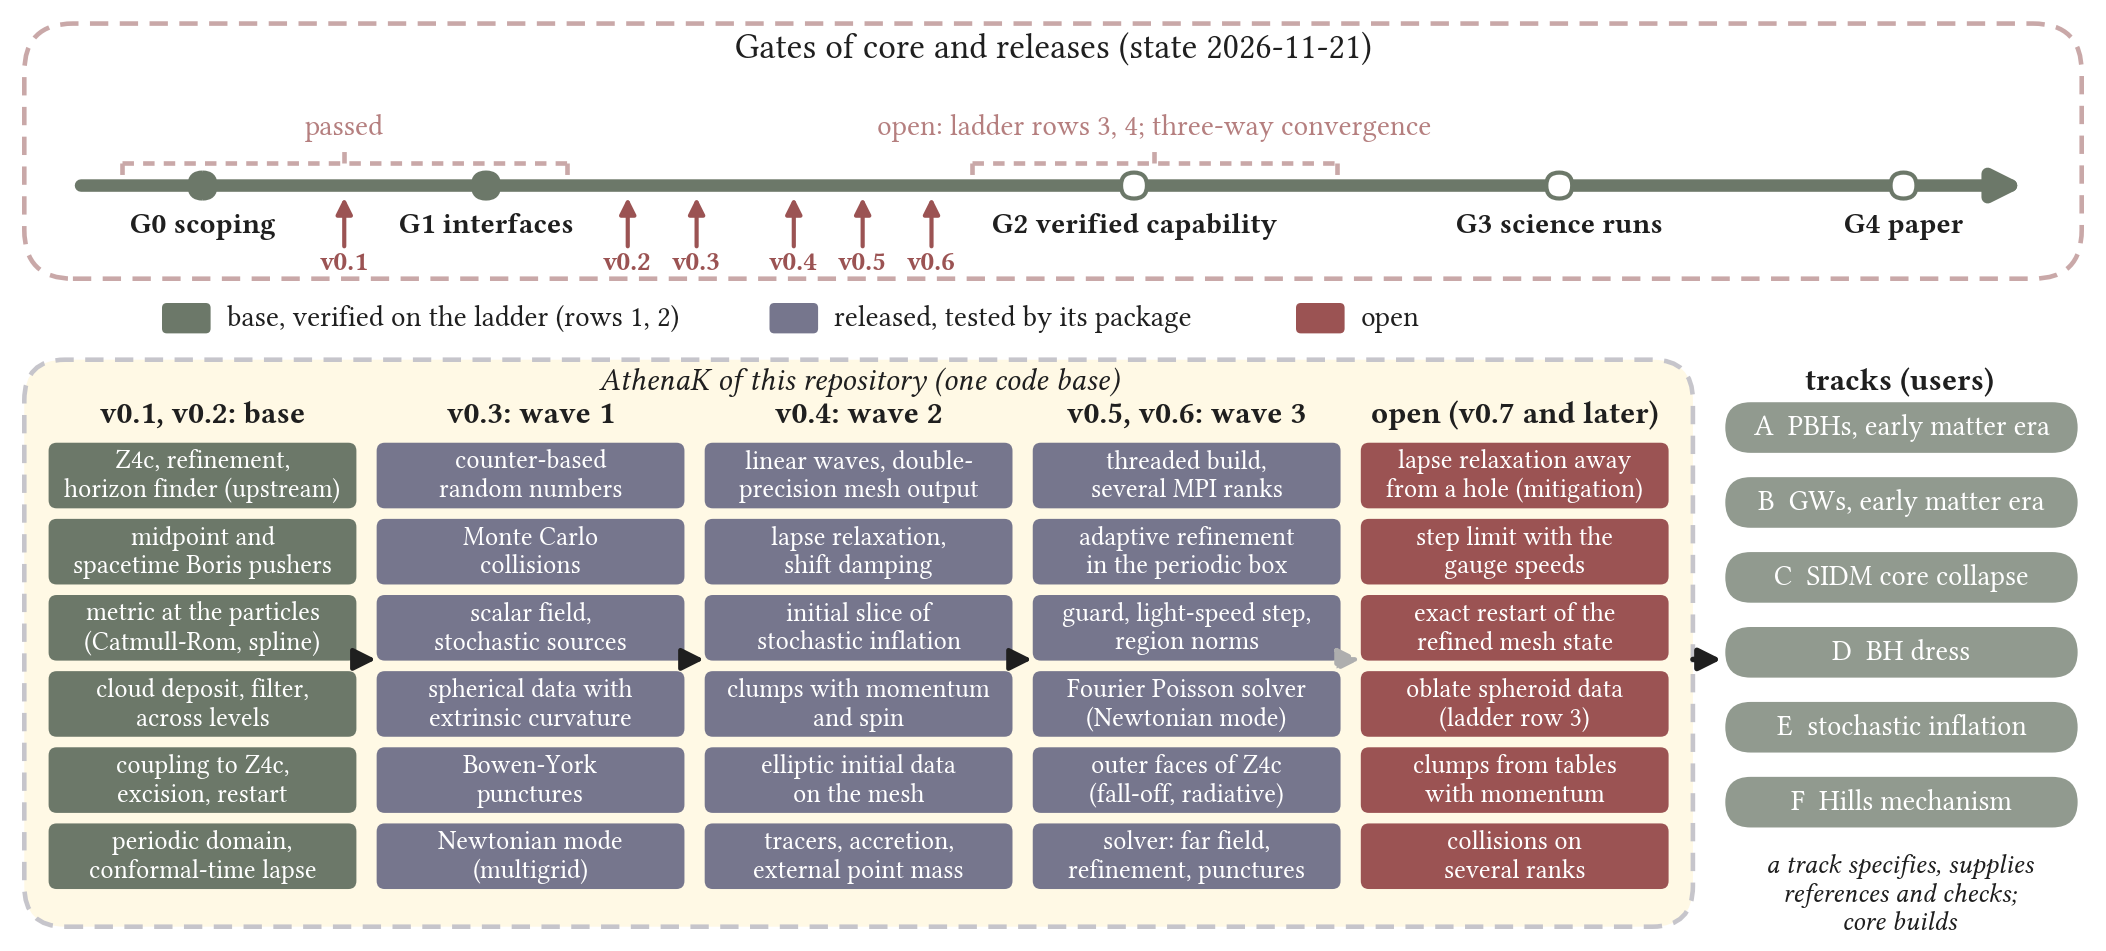
\includegraphics[width=\textwidth]{figures/schem_architecture.png}
\caption{The shared implementation by release (bottom) and the gates of the shared
implementation with the release tags (top). Green: the base, verified on the first two
rows of the ladder; slate: released capabilities, each tested by its own package; red:
open items. Arrows on the right lead to the six projects that use the code.}
\label{fig:arch}
\end{figure*}

\section{The verification ladder}\label{sec:ladder}

The brief of the program assigns four tests of its verification suite to the shared
implementation: geodesics on a fixed background; the Oppenheimer--Snyder collapse with a
horizon-mass error of the order of the source paper's; prolate collapse; and the
stability of relativistic clusters. Figures~\ref{fig:geo} to~\ref{fig:clusters} are
drawn from raw outputs by one registered run, which also writes the ledger of
Appendix~\ref{app:ledger}.

\subsection{Geodesics on a fixed Kerr background}

The test follows a bound geodesic of eccentricity $0.99$ past a Kerr black hole of spin
$a=0.9\,M$ in Kerr--Schild coordinates, with the metric either evaluated analytically at
the particle or interpolated from a lattice. Figure~\ref{fig:geo} shows the largest
relative errors of the energy, the axial angular momentum and the Carter constant along
the passage, from the regression of the merged processor build. Every largest error
equals the source paper's to the digits the paper prints; the midpoint rule keeps the
axial angular momentum to round-off. The final position error falls with the square of
the step for both pushers, and the pericentre agrees with the exact orbit. The row
passes; the comparison with the integrators named in the brief remains to be made.

\begin{figure*}
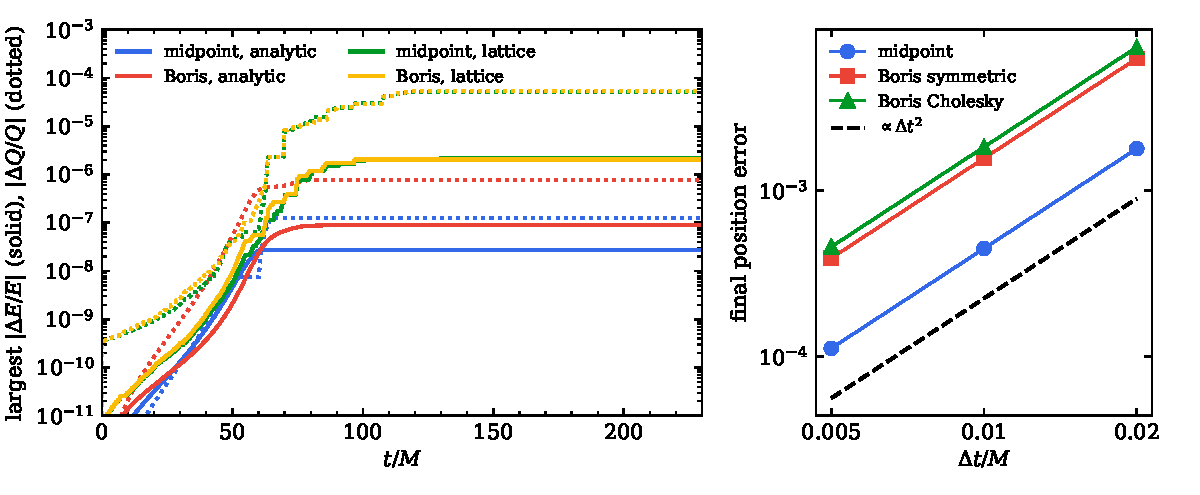
\includegraphics[width=\textwidth]{figures/fig_geodesic.pdf}
\caption{Kerr passage, $a=0.9\,M$, $e=0.99$. Left: running maximum of the relative error
of the energy (solid) and of the Carter constant (dotted) for the two pushers with the
analytic metric and with the interpolated lattice. Right: error of the final position
against the step for the three pushers with the analytic metric; dashed: the square of
the step.}
\label{fig:geo}
\end{figure*}

\subsection{Oppenheimer--Snyder collapse}

A homogeneous dust ball on a lattice of particles collapses from rest. The left panel of
Fig.~\ref{fig:collapse} shows the horizon mass $\Mah$ against time. When the horizon
forms, $\Mah$ equals the initial mass within the source paper's band, and the merged card
build reproduces the reference run until the end of its window, with an identical first
horizon. Later in the reference run the mass falls slowly below the band and stays just
outside it; the paper reaches its band with about a hundred times more particles. The
row passes on the criterion of the brief, an error of the order of the paper's. The
deposition identity, the equality of the mesh integral of the deposited energy and the
sum over the particles, holds to round-off throughout. Open: a sequence in particle
number with several random seeds, as in the paper's appendix.

\subsection{Oblate and prolate collapse}

A prolate spheroid of particles collapses into a spindle and forms a horizon. At finest
cells of $M/16$ and $M/8$ the first horizon appears at the paper's time within one search
interval (Fig.~\ref{fig:collapse}, right). Its mass stays a few hundredths below the
initial mass and falls slowly after its maximum; the deficit shrinks from the coarser to
the finer mesh, and the missing mass sits outside the horizon as field content. Two
resolutions give no order of convergence, and a third needs more memory than one card
holds at this particle number. The oblate member of the row has its initial-data component
on a branch scheduled for the next release. The row is partial.

\begin{figure*}
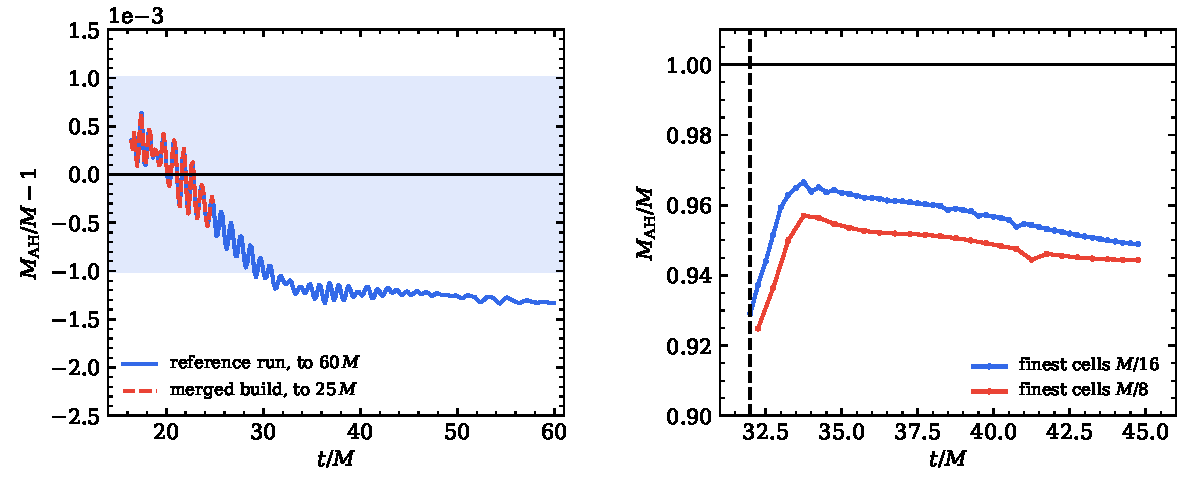
\includegraphics[width=\textwidth]{figures/fig_collapse.pdf}
\caption{Horizon masses. Left: Oppenheimer--Snyder collapse of a lattice of 9328
particles, $\Mah/M-1$ of the reference run and of the merged card build; shaded: the
source paper's level. Right: prolate collapse at two finest cell sizes; dashed: the
paper's first-horizon time.}
\label{fig:collapse}
\end{figure*}

\subsection{Steady states and the stability threshold}

The monoenergetic clusters of the paper form a sequence in the central parameter $y_c$;
the paper evolves five of them with a small inward kick. With $10^4$ particles on an
adaptive mesh, the two stable models keep their central lapse $\alpha_c$
within a narrow band and every particle, the models $y_c=0.605$ and $0.500$ collapse to
black holes whose horizon mass equals the cluster's mass, and $y_c=0.283$ expands
(Fig.~\ref{fig:clusters}, left). The fates agree with the paper; the collapse times are
longer than the paper's, which the paper itself calls dependent on particle number and
initial noise.

The threshold lies near the turning point of the binding energy along the sequence,
$y_c^\ast$. A bisection between the turning point and the collapsing model, on a mesh
capped at cells of $M/4$, found no collapse within the evolved time
(Fig.~\ref{fig:clusters}, right): members below $y_c^\ast$ moved to their partner of equal
binding energy, those above stayed, and the same initial data that collapsed on the finer
adaptive mesh migrated on the capped one. A collisionless cluster drifts outward on the
coarse mesh, and far less on cells of $M/8$, by the control runs of the
self-interacting-core project; an outward drift of that size stabilises a model. The
bisection is therefore repeated on cells of $M/8$, each member beside an unkicked control
on the same mesh, with the rule for its fate written before the runs: a run collapses
when a horizon appears or the central lapse falls below $0.3$ within $300\,M$; a member
that does not collapse stays when the mean of its central lapse over $200$--$300\,M$ lies
within $0.01$ of its control's mean.

On this mesh the collapse branch returns (Fig.~\ref{fig:row4m8}). The kicked model
$y_c=0.605$ collapses at $t_c=180.5\,M$, while its control moves outward, towards its
partner of equal binding energy. At $y_c=0.680$, which lies $0.0004$ above the turning
point, the member collapses at $219.5\,M$ and the control at $251.5\,M$, so the particle
noise alone suffices. At $y_c=0.755$ neither run collapses, and the two means differ by
$0.002$. On cells of $M/8$ with $10^4$ particles the threshold is therefore bracketed
between $y_c=0.680$ and $0.755$, and the turning point lies just below the bracket. That
a model this close to the turning point collapses from noise within $260\,M$ suggests
that the threshold of the discretised system lies above $y_c^\ast$, by up to $0.075$.
The controls drift on this mesh too: both runs at $y_c=0.755$ settle $0.025$ below the
equilibrium lapse, inward rather than outward, and $0.025$ is more than the $0.01$
predicted from the self-interacting-core controls. The next level of the bisection,
three models with their controls between $0.680$ and $0.755$, is in the queue. The
growing oscillation of the central lapse, $\pm0.03$ after $200\,M$ at $y_c=0.755$, is
still unexplained. The row is partial.

\begin{figure*}
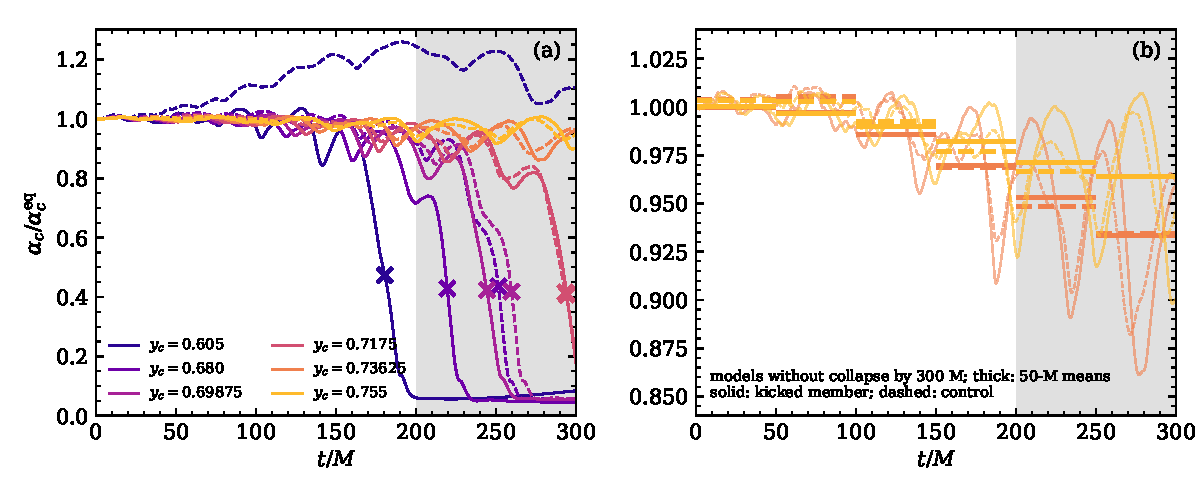
\includegraphics[width=\textwidth]{figures/fig_row4_m8.pdf}
\caption{Central lapse of the bisection on cells of $M/8$, first level. Solid lines show
the members with the one-per-cent inward kick and dashed lines the unkicked controls on
the same mesh. Dotted lines mark the equilibrium central lapse of each model, the grey
band the window $200$--$300\,M$ of the rule, and crosses the collapse time (central lapse
below $0.3$). Right: the runs without collapse on an expanded axis.}
\label{fig:row4m8}
\end{figure*}

\begin{figure*}
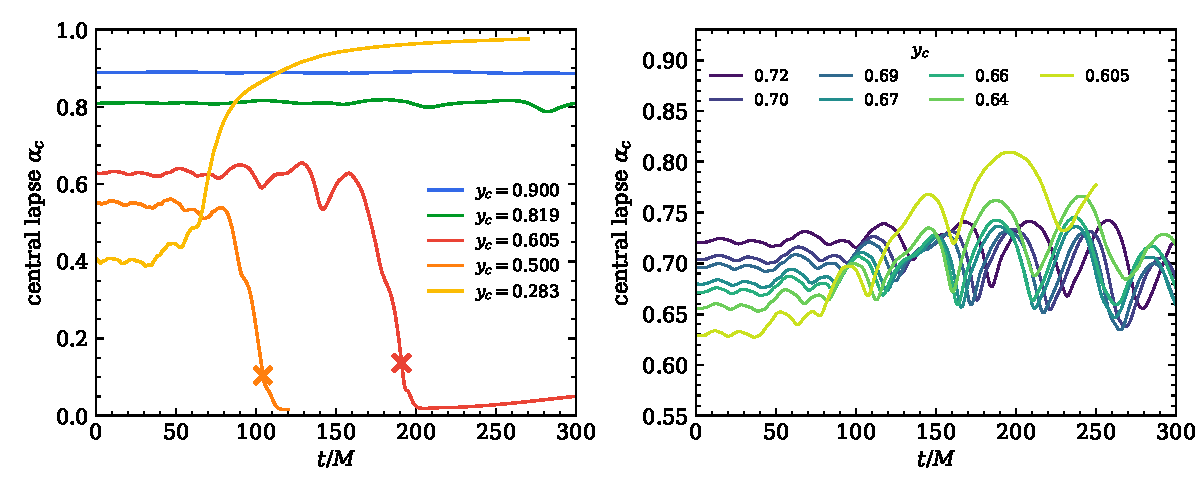
\includegraphics[width=\textwidth]{figures/fig_clusters.pdf}
\caption{Central lapse of the cluster models. Left: the five models of the paper's
sequence on the adaptive mesh; crosses mark the first apparent horizon. Right: the
bisection between the turning point and the collapsing model on a mesh capped at cells of
$M/4$, labelled by $y_c$; the last member is the unkicked control.}
\label{fig:clusters}
\end{figure*}

\subsection{Constraints, conservation and restarts}

In the homogeneous expanding universe the proper-volume integrals of the squared
Hamiltonian constraint and of the squared Z4c variable $\Theta$ stay small, as do their
pointwise values, and the lapse, the mean extrinsic curvature and the proper volume
follow the Einstein--de Sitter solution closely. Initial data solved on the mesh satisfy the
constraints to the tolerance of the solver on every refinement level, also after the
merge into the card build. With several MPI ranks the deposition identity and the
particle positions agree with one rank to round-off. A restart repeats a periodic run
byte for byte; with outflow faces and refinement it repeats the particle state exactly,
while the mesh state differs at round-off, so a chained run of an isolated system
repeats only up to the growth of round-off.

\subsection{Independent check}

A verifier with no part in this work, given the claims and the raw outputs but none of
the conclusions, recomputed fourteen claims with its own readers and references: every
met row of the ladder and at least one capability of each release. Twelve numbers agree
to their printed digits. The general statement that restarts are exact held only for
periodic set-ups and the particle state, as above. Five texts stated a measure or a count
loosely: a volume norm printed as a pointwise maximum, an absolute frequency difference
read as a relative one, a tracer count, an unstated relative error, and one rounded
digit. All five are corrected, and the ledger marks which of its rows the verifier
recomputed.

\section{Known limits}\label{sec:limits}

The lapse relaxation of the second release holds the lapse wherever it exceeds its
reference value, matter or vacuum. Around a black hole in vacuum the horizon then
shrinks in coordinates and its mass drifts late in the run, well beyond the band of the
same run without the relaxation, as the black-hole-dress project found. Null tests and
long runs around an existing black hole therefore run without it. The next release
switches the term off inside a radius around each tracked puncture; this delays the
drift and is named a mitigation. A cure, a term that holds the lapse of expanding matter
without stretching the vacuum, is open.

The step limit counts the speed of light only. The primordial
black-hole project found the Gamma-driver shift unstable at the grid scale once the step
exceeds a fixed fraction of the finest cell; the rule until the next release keeps the
Courant factor below that fraction, and the next release adds the gauge speeds to the
step limit.

Further limits are on record with their tests: restarts of refined isolated systems
repeat the mesh state at round-off only; the new outer faces reduce the reflection of
the constraint layer without removing it; the second pass of the elliptic solver stalls
in its vector part at level boundaries; and in the Newtonian mode a cold lattice coarser
than the mesh is pushed by the self-forces of its own particles.

\section{Summary}

The base coupling passes the first two rows of the verification ladder on the merged and
released executables, and four releases added what six projects asked for, each with its
own tests and an interface document. The numbers of the ladder and of a sample of every
release survive an independent recomputation from raw outputs. For the gate the shared
implementation still needs: the oblate initial data in a release and its collapse, a
third resolution or a particle-number pair for the prolate collapse, the stability
threshold narrowed on the finer mesh (it is bracketed there, between $y_c=0.680$ and
$0.755$, but not yet converged in cell size or particle number), and one coupled set-up converged
in particle number, cell size and gauge together.

\appendix

\onecolumngrid
\section{Numerical ledger}\label{app:ledger}

Every number of this note, with the registered run that produced it or the source line
it was read from, and the claim of the independent verifier (V1 to V11 of its report)
where it recomputed the number from raw outputs. Rows of the four data sections were
written by the run that made the figures (\noterun); the other rows are copied from the
documents of the stage package with their runs. Runs whose identifier begins with a path
are older than the program's run registry; their files are inventoried by checksum in
run \texttt{core-20261121-231825-135474c}.

{\small
\begin{longtable}{@{}r p{0.46\textwidth} p{0.15\textwidth} p{0.25\textwidth} l@{}}
\hline\hline
\# & Quantity & Value & Source & Verifier\\ \hline
\endhead
\hline\hline
\endlastfoot
\multicolumn{5}{@{}l}{\textit{Row 1: Kerr passage, a = 0.9 M, e = 0.99, dt = 0.01 M to 230 M (regression G)}}\\
1 & E at t = 0 & 0.99738 & \texttt{\footnotesize core-20261115-065452-3629622} & V1\\
2 & L\_z at t = 0 & 2.4328 & \texttt{\footnotesize core-20261115-065452-3629622} & V1\\
3 & Q at t = 0 & 1.974 & \texttt{\footnotesize core-20261115-065452-3629622} & V1\\
4 & midpoint, analytic metric: largest $|$dE/E$|$ & 2.781e-08 & \texttt{\footnotesize core-20261115-065452-3629622} & V1\\
5 & midpoint, analytic metric: largest $|$dL\_z/L\_z$|$ & 0 & \texttt{\footnotesize core-20261115-065452-3629622} & V1\\
6 & midpoint, analytic metric: largest $|$dQ/Q$|$ & 1.254e-07 & \texttt{\footnotesize core-20261115-065452-3629622} & V1\\
7 & Boris symmetric, analytic: largest $|$dE/E$|$ & 9.046e-08 & \texttt{\footnotesize core-20261115-065452-3629622} & V1\\
8 & Boris symmetric, analytic: largest $|$dL\_z/L\_z$|$ & 1.136e-08 & \texttt{\footnotesize core-20261115-065452-3629622} & V1\\
9 & Boris symmetric, analytic: largest $|$dQ/Q$|$ & 7.825e-07 & \texttt{\footnotesize core-20261115-065452-3629622} & V1\\
10 & midpoint, Hermite lattice: largest $|$dE/E$|$ & 2.162e-06 & \texttt{\footnotesize core-20261115-065452-3629622} & V1\\
11 & midpoint, Hermite lattice: largest $|$dL\_z/L\_z$|$ & 5.304e-06 & \texttt{\footnotesize core-20261115-065452-3629622} & V1\\
12 & midpoint, Hermite lattice: largest $|$dQ/Q$|$ & 5.060e-05 & \texttt{\footnotesize core-20261115-065452-3629622} & V1\\
13 & Boris Cholesky, lattice: largest $|$dE/E$|$ & 2.046e-06 & \texttt{\footnotesize core-20261115-065452-3629622} & V1\\
14 & Boris Cholesky, lattice: largest $|$dL\_z/L\_z$|$ & 3.788e-06 & \texttt{\footnotesize core-20261115-065452-3629622} & V1\\
15 & Boris Cholesky, lattice: largest $|$dQ/Q$|$ & 5.289e-05 & \texttt{\footnotesize core-20261115-065452-3629622} & V1\\
16 & midpoint: order in dt of the final position error (0.005-0.01) & 2.0001 & \texttt{\footnotesize core-20261115-065452-3629622} & V1\\
17 & midpoint: same (0.01-0.02) & 2.0003 & \texttt{\footnotesize core-20261115-065452-3629622} & V1\\
18 & Boris symmetric: order (0.005-0.01) & 1.9998 & \texttt{\footnotesize core-20261115-065452-3629622} & V1\\
19 & Boris symmetric: order (0.01-0.02) & 1.9991 & \texttt{\footnotesize core-20261115-065452-3629622} & V1\\
20 & Boris Cholesky: order (0.005-0.01) & 1.9997 & \texttt{\footnotesize core-20261115-065452-3629622} & V1\\
21 & Boris Cholesky: order (0.01-0.02) & 1.9989 & \texttt{\footnotesize core-20261115-065452-3629622} & V1\\
22 & pericentre radius (M) & 1.898325 & \texttt{\footnotesize core-20261115-065452-3629622} & V1\\
23 & pericentre time (M) & 98.949 & \texttt{\footnotesize core-20261115-065452-3629622} & V1\\
\multicolumn{5}{@{}l}{\textit{Row 2: Oppenheimer-Snyder collapse, lattice of 9328 particles}}\\
24 & particles at t = 0 & 9328 & \texttt{\footnotesize runs/os/nocap\_sc (pre-program; inventory core-20261121-231825-135474c)} & V2\\
25 & reference run: first apparent horizon (M) & 16.3894 & \texttt{\footnotesize runs/os/nocap\_sc (pre-program; inventory core-20261121-231825-135474c)} & V2\\
26 & reference run: M\_AH/M at formation & 1.000353 & \texttt{\footnotesize runs/os/nocap\_sc (pre-program; inventory core-20261121-231825-135474c)} & V2\\
27 & reference run: largest $|$M\_AH/M - 1$|$ to 60 M & 0.001338 & \texttt{\footnotesize runs/os/nocap\_sc (pre-program; inventory core-20261121-231825-135474c)} & V2\\
28 & reference run: M\_AH/M near 20 M (search at 20.023 M) & 1.000093 & \texttt{\footnotesize runs/os/nocap\_sc (pre-program; inventory core-20261121-231825-135474c)} & V2\\
29 & reference run: M\_AH/M near 40 M (search at 40.008 M) & 0.9987625 & \texttt{\footnotesize runs/os/nocap\_sc (pre-program; inventory core-20261121-231825-135474c)} & V2\\
30 & reference run: M\_AH/M near 60 M (search at 59.994 M) & 0.9986707 & \texttt{\footnotesize runs/os/nocap\_sc (pre-program; inventory core-20261121-231825-135474c)} & V2\\
31 & reference run: first search with $|$M\_AH/M - 1$|$ $>$ 1e-3 (M) (first search with $|$M\_AH/M - 1$|$ above 1e-3) & 29.11 & \texttt{\footnotesize runs/os/nocap\_sc (pre-program; inventory core-20261121-231825-135474c)} & V2\\
32 & reference run: above 1e-3 at every search from (M) (first search after which every search has $|$M\_AH/M - 1$|$ above 1e-3) & 30.92 & \texttt{\footnotesize runs/os/nocap\_sc (pre-program; inventory core-20261121-231825-135474c)} & V2\\
33 & reference run: all particles removed by (M) & 19.74 & \texttt{\footnotesize runs/os/nocap\_sc (pre-program; inventory core-20261121-231825-135474c)} & V2\\
34 & merged card build: first apparent horizon (M) & 16.3894 & \texttt{\footnotesize core-20261115-065901-3629622} & V2\\
35 & merged card build: M\_AH/M at formation & 1.000353 & \texttt{\footnotesize core-20261115-065901-3629622} & V2\\
36 & merged card build: largest $|$M\_AH/M - 1$|$ to 25 M & 6.345e-04 & \texttt{\footnotesize core-20261115-065901-3629622} & V2\\
\multicolumn{5}{@{}l}{\textit{Row 3: prolate collapse, 10$^4$ particles}}\\
37 & finest cells M/16: first apparent horizon (M) & 32 & \texttt{\footnotesize runs/prolate/e09\_v8 (pre-program; inventory core-20261121-231825-135474c)} & \\
38 & M/16: M\_AH/M at formation & 0.9291 & \texttt{\footnotesize runs/prolate/e09\_v8 (pre-program; inventory core-20261121-231825-135474c)} & \\
39 & M/16: largest M\_AH/M & 0.9666 & \texttt{\footnotesize runs/prolate/e09\_v8 (pre-program; inventory core-20261121-231825-135474c)} & \\
40 & M/16: M\_AH/M at the last search (44.75 M) & 0.9489 & \texttt{\footnotesize runs/prolate/e09\_v8 (pre-program; inventory core-20261121-231825-135474c)} & \\
41 & finest cells M/8: first apparent horizon (M) & 32.25 & \texttt{\footnotesize core-20261115-152845-5728b1d} & \\
42 & M/8: M\_AH/M at formation & 0.9249 & \texttt{\footnotesize core-20261115-152845-5728b1d} & \\
43 & M/8: largest M\_AH/M & 0.957 & \texttt{\footnotesize core-20261115-152845-5728b1d} & \\
44 & M/8: M\_AH/M at the last search (44.75 M) & 0.9444 & \texttt{\footnotesize core-20261115-152845-5728b1d} & \\
\multicolumn{5}{@{}l}{\textit{Row 4: cluster sequence, 10$^4$ particles, one-per-cent inward kick}}\\
45 & y\_c = 0.900: smallest central lapse to 300 M & 0.8862 & \texttt{\footnotesize runs/st/yc0900\_v4 (pre-program; inventory core-20261121-231825-135474c)} & V3\\
46 & y\_c = 0.900: largest central lapse to 300 M & 0.8919 & \texttt{\footnotesize runs/st/yc0900\_v4 (pre-program; inventory core-20261121-231825-135474c)} & V3\\
47 & y\_c = 0.900: particles kept (of 10$^4$) & 10000 & \texttt{\footnotesize runs/st/yc0900\_v4 (pre-program; inventory core-20261121-231825-135474c)} & V3\\
48 & y\_c = 0.819: smallest central lapse to 300 M & 0.7875 & \texttt{\footnotesize runs/st/yc0819\_v4 (pre-program; inventory core-20261121-231825-135474c)} & V3\\
49 & y\_c = 0.819: largest central lapse to 300 M & 0.819 & \texttt{\footnotesize runs/st/yc0819\_v4 (pre-program; inventory core-20261121-231825-135474c)} & V3\\
50 & y\_c = 0.819: particles kept & 10000 & \texttt{\footnotesize runs/st/yc0819\_v4 (pre-program; inventory core-20261121-231825-135474c)} & V3\\
51 & y\_c = 0.605: first apparent horizon (M) & 191 & \texttt{\footnotesize runs/st/yc0605\_v5 (pre-program; inventory core-20261121-231825-135474c)} & V3\\
52 & y\_c = 0.605: M\_AH/M at the end & 0.99999 & \texttt{\footnotesize runs/st/yc0605\_v5 (pre-program; inventory core-20261121-231825-135474c)} & V3\\
53 & y\_c = 0.500: first apparent horizon (M) & 104.31 & \texttt{\footnotesize runs/st/yc0500\_v5 (pre-program; inventory core-20261121-231825-135474c)} & V3\\
54 & y\_c = 0.500: M\_AH/M at the end & 1.0001 & \texttt{\footnotesize runs/st/yc0500\_v5 (pre-program; inventory core-20261121-231825-135474c)} & V3\\
55 & y\_c = 0.283: central lapse at 270 M (record at 270.00 M) & 0.97598 & \texttt{\footnotesize runs/st/yc0283\_v5 (pre-program; inventory core-20261121-231825-135474c)} & V3\\
56 & y\_c = 0.283: particles kept & 10000 & \texttt{\footnotesize runs/st/yc0283\_v5 (pre-program; inventory core-20261121-231825-135474c)} & V3\\
57 & M/4 bisection, y\_c = 0.72: mean central lapse 200-300 M & 0.7079 & \texttt{\footnotesize core-20261115-152843-5728b1d} & V3\\
58 & y\_c = 0.70: same & 0.692 & \texttt{\footnotesize core-20261115-152842-5728b1d} & \\
59 & y\_c = 0.69: same & 0.6864 & \texttt{\footnotesize core-20261115-154726-37450f2} & \\
60 & y\_c = 0.67: same & 0.6911 & \texttt{\footnotesize core-20261115-154726-37450f2} & \\
61 & y\_c = 0.66: same & 0.7005 & \texttt{\footnotesize core-20261115-152842-5728b1d} & \\
62 & y\_c = 0.64: same & 0.7221 & \texttt{\footnotesize core-20261115-152843-5728b1d} & \\
63 & control y\_c = 0.605: mean central lapse 200-250 M & 0.7667 & \texttt{\footnotesize core-20261115-155617-06f844b} & \\
\multicolumn{5}{@{}l}{\textit{Row 4 on cells of M/8, level 1 (member kicked, control unkicked; rule of JOURNAL 2026-11-21T20:26Z)}}\\
64 & y\_c = 0.605: equilibrium central lapse & 0.6281 & \texttt{\footnotesize core-20261121-202643-d66c4ee} & \\
65 & y\_c = 0.605 member: collapse time t\_c (M) & 180.5 & \texttt{\footnotesize core-20261121-204230-3bcb118} & \\
66 & y\_c = 0.605 member: first apparent horizon (M) & 188 & \texttt{\footnotesize core-20261121-204230-3bcb118} & \\
67 & y\_c = 0.605 control: mean central lapse 200-300 M & 0.7303 & \texttt{\footnotesize core-20261121-204235-0b25077} & \\
68 & y\_c = 0.680: equilibrium central lapse & 0.6875 & \texttt{\footnotesize core-20261121-202643-d66c4ee} & \\
69 & y\_c = 0.680 member: collapse time t\_c (M) & 219.5 & \texttt{\footnotesize core-20261121-204234-d010783} & \\
70 & y\_c = 0.680 member: first apparent horizon (M) & 225 & \texttt{\footnotesize core-20261121-204234-d010783} & \\
71 & y\_c = 0.680 control: collapse time t\_c (M) & 251.5 & \texttt{\footnotesize core-20261121-204239-2be5ac2} & \\
72 & y\_c = 0.680 control: first apparent horizon (M) & 256 & \texttt{\footnotesize core-20261121-204239-2be5ac2} & \\
73 & y\_c = 0.755: equilibrium central lapse & 0.7509 & \texttt{\footnotesize core-20261121-202643-d66c4ee} & \\
74 & y\_c = 0.755 member: mean central lapse 200-300 M & 0.7264 & \texttt{\footnotesize core-20261121-204232-f74c942} & \\
75 & y\_c = 0.755 control: mean central lapse 200-300 M & 0.7247 & \texttt{\footnotesize core-20261121-204237-ae00ca2} & \\
76 & y\_c = 0.755: D = member minus control mean & 0.0016 & \texttt{\footnotesize core-20261121-204232-f74c942 - core-20261121-204237-ae00ca2} & \\
\multicolumn{5}{@{}l}{\textit{Paper (Wu and Most), read with line locators}}\\
77 & Kerr passage, midpoint analytic: largest errors E, L\_z, Q & 2.8e-8, round-off, 1.3e-7 & \texttt{\footnotesize paper main.tex 824-833} & \\
78 & Kerr passage, Boris Cholesky lattice: same & 2.0e-6, 3.8e-6, 5.3e-5 & \texttt{\footnotesize paper main.tex 824-833} & \\
79 & Oppenheimer-Snyder: relative horizon-mass error & $\lesssim$ 1e-3 & \texttt{\footnotesize paper main.tex 945} & \\
80 & Oppenheimer-Snyder fiducial lattice particles & 998592 & \texttt{\footnotesize paper main.tex 917} & \\
81 & prolate collapse: first apparent horizon (M) & 32 & \texttt{\footnotesize paper main.tex 971} & \\
82 & clusters y\_c = 0.605, 0.500: first horizons (M) & 109, 73 & \texttt{\footnotesize paper main.tex 1138} & \\
83 & migration of y\_c = 0.5: late mean central lapse & 0.833530 & \texttt{\footnotesize paper main.tex 1199} & \\
\multicolumn{5}{@{}l}{\textit{Turning point and bisection protocol}}\\
84 & turning point of the sequence y\_c* & 0.6796 & \texttt{\footnotesize core-20261115-152805-47d8f25} & \\
85 & E\_b/M\_0 at y\_c* & 0.036058 & \texttt{\footnotesize core-20261115-152805-47d8f25} & \\
86 & card time of the seven M/4 bisection runs (card-hours) & 2.0 & \texttt{\footnotesize verify/LADDER.md row 4, wave 2} & \\
\multicolumn{5}{@{}l}{\textit{Constraints and conservation (C3)}}\\
87 & homogeneous universe: H-norm2 (proper-volume integral of H$^2$) & 3.7e-10 & \texttt{\footnotesize core-20261115-065903-3629622} & V4\\
88 & homogeneous universe: Theta-norm2 (proper-volume integral of Theta$^2$) & 1.1e-11 & \texttt{\footnotesize core-20261115-065903-3629622} & V4\\
89 & homogeneous universe: pointwise max$|$Theta$|$, max$|$H$|$ & 2.27e-7, 1.69e-6 & \texttt{\footnotesize core-20261121-212248-a7972d1} & V4\\
90 & homogeneous universe against Einstein-de Sitter: lapse, mean K, proper volume (relative) & 1.9e-7, 3.8e-7, 1.1e-6 & \texttt{\footnotesize core-20261121-212248-a7972d1} & V4\\
91 & dust collapse: deposition identity (mesh integral against particle sum) & 1.0e-15 & \texttt{\footnotesize core-20261115-065901-3629622} & V5a\\
92 & MPI, periodic cosmology on 2, 4 ranks: particle positions against one rank & 1.6e-14 & \texttt{\footnotesize core-20261119-163641-ddb47b0} & V5b\\
93 & MPI, periodic cosmology on 1, 2, 4 ranks: deposition identity & 1e-14 & \texttt{\footnotesize core-20261119-163641-ddb47b0} & V5b\\
94 & Bowen-York puncture after the solve, card and processor: max$|$H$|$ & 6.4e-12 & \texttt{\footnotesize core-20261121-154700-2de4974} & \\
\multicolumn{5}{@{}l}{\textit{Restart (fresh verifier, release core-v0.6 processor build)}}\\
95 & periodic Z4c, 4096 particles, restart at cycle 10 of 20: differing bytes & 0 & \texttt{\footnotesize core-20261121-213713-952a0c4} & V6\\
96 & Oppenheimer-Snyder, refinement, outflow faces, restart at cycle 3 of 6: mesh words differing & 64 per cent & \texttt{\footnotesize core-20261121-215228-d1f36f4} & V6\\
97 & same: median, 99th percentile of the relative difference & 2.8e-13, 1.7e-7 & \texttt{\footnotesize core-20261121-215228-d1f36f4} & V6\\
98 & same: histories within & 5e-13 & \texttt{\footnotesize core-20261121-215228-d1f36f4} & V6\\
\multicolumn{5}{@{}l}{\textit{Capabilities of core-v0.3 to core-v0.6 (package runs; verifier's rerun where named)}}\\
99 & v0.3 Newtonian point mass: rms relative force error at N = 32, 64; order & 1.61e-2, 4.94e-3; 1.70 & \texttt{\footnotesize core-20261115-150209-3629622} & V7a\\
100 & same: tracers at r $\geq$ 0.5 & 706 & \texttt{\footnotesize core-20261121-212516-0f0a65b} & V7a\\
101 & v0.3 collisions, box relaxation: Kolmogorov-Smirnov p of the four end states & 0.26 to 0.90 & \texttt{\footnotesize core-20261115-134036-5684674} & V8\\
102 & v0.3 scalar field test 1a: spatial orders for nghost 2, 3, 4 & 1.991, 3.957, 5.918 & \texttt{\footnotesize core-20261115-150004-3629622} & V9\\
103 & same: Omega/omega\_h - 1 at dt = 1/512 & -1.21e-9 to -1.31e-9 & \texttt{\footnotesize core-20261121-212422-b616c6e} & V9\\
104 & v0.4 solver T1: relative error of psi - 1 at the centre, code, dx = 1, 0.5, 0.25 & -1.92e-2, -5.22e-3, -1.33e-3 & \texttt{\footnotesize core-20261121-214108-0960a46} & V10a\\
105 & v0.6 solver on static refinement: relative error of psi - 1 over r $<$ 1, refined against uniform & -5.01e-3, -5.03e-3 & \texttt{\footnotesize core-20261119-153510-d1eaa30} & V10b\\
106 & v0.6 Fourier solver, exact pancake: slab I\_xx error, spectral and seven-point & 9.1e-6, 3.1e-3 & \texttt{\footnotesize core-20261119-160919-c6a7279} & V7b\\
107 & v0.6 faces: stock boundary-layer $|$H$|$ over the stencil estimate & 0.79 & \texttt{\footnotesize core-20261119-143938-eded041} & V11\\
108 & v0.6 faces: reduction of the layer by the fall-off ghosts & 12 & \texttt{\footnotesize core-20261121-214547-7a21ed3} & V11\\
109 & byte regression of v0.6 against v0.5 & 75 of 75 & \texttt{\footnotesize core-20261121-130202-7cf7db8} & \\
110 & byte regression of v0.5 against v0.4 & PASS & \texttt{\footnotesize core-20261121-063859-e410ee3} & \\
111 & byte regression of v0.4 against v0.3 & PASS & \texttt{\footnotesize core-20261120-221607-4985804} & \\
112 & card check of the merged v0.6 card build: cases & 15, PASS & \texttt{\footnotesize core-20261121-154700-2de4974} & \\
\multicolumn{5}{@{}l}{\textit{Known defects (numbers of other owners, not recomputed by core)}}\\
113 & relaxed lapse, vacuum puncture: horizon-mass band 100-199.5 M with lapse\_leak = 0.5 & -5.6e-4 to +1.27e-3 & \texttt{\footnotesize D-20261121-125909-06f856e, D-20261121-144657-cf510fc} & \\
114 & same without the option & -4.8e-5 to +2.0e-5 & \texttt{\footnotesize D-20261121-125909-06f856e, D-20261121-144657-cf510fc} & \\
115 & Gamma-driver shift: stability bound dt/dx (nghost 4, RK4, dissipation 0.5) & 0.685 & \texttt{\footnotesize A-20261121-212800-d7f31a4} & \\
116 & rule until the step limit counts the gauge speeds: cfl\_number at most & 0.6 & \texttt{\footnotesize coord/DECISIONS/0027 item 2} & \\
\end{longtable}

}

\twocolumngrid
\bibliography{references}

\end{document}
